\documentclass[11pt]{article}

% ---------- Packages ----------
\usepackage[a4paper,margin=1in]{geometry}
\usepackage[T1]{fontenc}
\usepackage[utf8]{inputenc}
\usepackage{lmodern}
\usepackage{graphicx}
\usepackage{float}
\usepackage{booktabs}
\usepackage{caption}
\captionsetup{font=footnotesize}
\usepackage{microtype}
\usepackage{amsmath}
\usepackage{fontawesome5}
\usepackage{hyperref}
\usepackage[nameinlink]{cleveref}
\usepackage[superscript]{cite}
\usepackage{bookmark}
\bookmarksetup{numbered}
\usepackage{enumitem}
\usepackage{setspace}
\onehalfspacing
\usepackage{tabularx}
\usepackage{fancyhdr}
\usepackage{tikz}
\usepackage{placeins}
\usetikzlibrary{arrows.meta, positioning}
\setcounter{tocdepth}{2}
\renewcommand{\contentsname}{Contents}

% ---------- Header and Footer ----------
\pagestyle{fancy}
\fancyhf{}
\fancyhead[L]{The Hebrew University of Jerusalem}
\fancyhead[R]{Computational Genomics (76553)}
\fancyfoot[L]{\thepage}
\renewcommand{\headrulewidth}{0.4pt}
\renewcommand{\footrulewidth}{0.4pt}
\setlength{\headheight}{14pt}

\fancypagestyle{plain}{%
  \fancyhf{}
  \fancyhead[L]{The Hebrew University of Jerusalem}
  \fancyhead[R]{Computational Genomics (76553)}
  \fancyfoot[L]{\thepage}
  \renewcommand{\headrulewidth}{0.4pt}
  \renewcommand{\footrulewidth}{0.4pt}
}

% ---------- Metadata ----------
\hypersetup{
  pdftitle={Hide and Peak: Identifying MASLD-associated regulatory genes from cell-type chromatin accessibility},
  pdfauthor={Or Forshmit, Dvir Mateless, Noam Kimhi},
  pdfsubject={Computational Genomics hackathon report},
  pdfkeywords={MASLD, MASH, snATAC-seq, chromatin accessibility, eQTL, ABC model, peak-to-gene}
}

\title{\textbf{Hide and Peak}\\Identifying MASLD-associated regulatory genes from cell-type chromatin accessibility}
\author{}
\date{}

\begin{document}
  \maketitle
  \vspace{-45pt}

  \begin{center}
    \renewcommand{\arraystretch}{1.15}
    \setlength{\tabcolsep}{3pt}

    \begin{tabular}{ccc}
      \begin{minipage}[t]{0.32\textwidth}\centering
        \textbf{Or Forshmit}\\[-1pt]
        \footnotesize\href{mailto:or.forshmit@mail.huji.ac.il}{\texttt{or.forshmit@mail.huji.ac.il}}
      \end{minipage}
      &
      \begin{minipage}[t]{0.32\textwidth}\centering
        \textbf{Dvir Mateless}\\[-1pt]
        \footnotesize\href{mailto:dvir.mateless@mail.huji.ac.il}{\texttt{dvir.mateless@mail.huji.ac.il}}
      \end{minipage}
      &
      \begin{minipage}[t]{0.32\textwidth}\centering
        \textbf{Noam Kimhi}\\[-1pt]
        \footnotesize\href{mailto:noam.kimhi@mail.huji.ac.il}{\texttt{noam.kimhi@mail.huji.ac.il}}
      \end{minipage}
    \end{tabular}

    \vspace{20pt}

    \href{https://github.com/noam-kimhi/Comp-Genomics-Hackathon}{\Large \faGithub} \\[5pt]
    \today
  \end{center}

  \tableofcontents
  \newpage

  \section{Introduction}\label{sec:introduction}

  \subsection{Background}\label{subsec:background}
  Metabolic dysfunction-associated steatotic liver disease (MASLD), and its inflammatory form MASH, are strongly influenced by noncoding genetic and epigenomic variation.
  A major challenge is that many disease-associated variants lie outside protein-coding genes, so their functional impact must be inferred through regulatory activity, chromatin state, and links between regulatory elements and target genes.
  The motivating study by Zhu et al. used single-nucleus ATAC-seq (snATAC-seq), liver eQTLs, and regulatory perturbation evidence to interpret metabolic liver disease risk alleles at cell-type resolution\cite{Zhu2026MetabolicLiver}.

  Our project starts from a complementary question.
  Instead of asking only which known variants influence expression, we ask whether disease-associated chromatin accessibility peaks can reveal biologically plausible MASLD genes even after removing peaks that overlap known significant liver eQTL variants.
  This is useful because a regulatory peak can be disease-relevant without being represented in a particular eQTL catalogue, especially when the signal is cell-type-specific, condition-dependent, or mediated through enhancer activity not captured by bulk liver expression data.

  \subsection{Research Question}\label{subsec:research-question}
  Can cell-type-specific chromatin accessibility peaks reveal MASLD-associated regulatory regions and candidate target genes that are not captured by known significant liver eQTLs?

  \subsection{Hypothesis}\label{subsec:hypothesis}
  We hypothesize that some MASH-associated regulatory changes are visible as differential chromatin accessibility in specific liver cell types.
  After filtering out peaks overlapping significant liver eQTL variants, the remaining peaks should still contain regulatory signals that can be mapped to biologically meaningful target genes using enhancer-gene linking.

  \subsection{Objectives}\label{subsec:objectives}
  \begin{itemize}[noitemsep, topsep=0pt]
    \item Process snATAC-seq peak-count matrices from healthy and MASH liver samples
    \item Create a shared consensus peak coordinate system across samples
    \item Split accessibility matrices by annotated cell type and aggregate them into pseudobulk profiles
    \item Identify differentially accessible peaks between healthy and MASH samples using DESeq2
    \item Remove peaks overlapping significant GTEx liver eQTL variants
    \item Map the remaining peaks to candidate target genes using Activity-by-Contact (ABC) predictions
    \item Interpret top candidate genes using external biological evidence
  \end{itemize}

  \section{Data}
  \label{sec:data}

  \subsection{snATAC-seq Samples}\label{subsec:snatac-seq-samples}
  The primary data consist of snATAC-seq peak-count matrices from \href{https://www.ncbi.nlm.nih.gov/geo/query/acc.cgi?acc=GSE281367}{\underline{GSE281367}}, downloaded through the \href{https://www.ncbi.nlm.nih.gov/geo/download/?acc=GSE281367&format=file}{\underline{GEO file download endpoint}}\cite{GSE281367}.
  The local \href{https://github.com/noam-kimhi/Comp-Genomics-Hackathon/tree/main/data/snatac_gse281367}{\path{data/snatac_gse281367/}} directory contains 12 human liver samples: six healthy and six MASH.
  Each sample directory contains barcodes, genomic peak coordinates, and a sparse accessibility matrix in Matrix Market format.
  These files define the raw chromatin-accessibility observations used throughout the project.

  The corresponding metadata and Seurat-derived annotations were used to assign nuclei to liver cell types.
  Specifically, we used the clustered Seurat object \href{https://www.ncbi.nlm.nih.gov/geo/download/?acc=GSE281367&format=file&file=GSE281367%5Fseurat%5Fclustered%2Erds%2Egz}{\underline{\path{GSE281367_seurat_clustered.rds.gz}}}, downloaded from GEO.
  Seurat is a widely used R framework for single-cell data integration, clustering, visualization, and annotation\cite{Hao2021Seurat}.
  In this project, we did not recluster the nuclei from scratch; rather, we extracted and reconciled the available Seurat annotations with the barcode-level matrix files so that each accessibility matrix could be split by cell type.

  Across the raw sample summaries, the MASH samples contained 78,124 cells and the healthy samples contained 57,067 cells.
  Median cells per sample were 11,988 for MASH and 9,296 for healthy samples.
  The sample-level peak sets varied substantially in size and boundary definitions, which motivated the consensus-peak construction described in \cref{subsec:consensus-peak-construction}.

  The analysis considered seven annotated cell-type groups: cholangiocytes, endothelial cells, hepatocytes, Kupffer cells, stellate cells, T/NK/B cells, and unknown cells.
  Pseudobulk matrices were generated separately for each cell type, each over the same reproducible consensus peak universe of 206,989 peaks.
  Because some cell types were absent or too sparse in individual samples, the number of samples with data ranged from 10 to 11 across cell-type-specific pseudobulk matrices.

  \subsection{External Regulatory Data}\label{subsec:external-regulatory-data}
  We used significant liver eQTL variant-gene pairs from \href{https://storage.googleapis.com/adult-gtex/bulk-qtl/v8/single-tissue-cis-qtl/GTEx_Analysis_v8_eQTL.tar}{\underline{GTEx v8}} to identify peaks already overlapping known liver eQTL variants\cite{GTEx2020}.
  These overlaps were used as a filter, not as a peak-to-gene mapping source: the goal was to focus on differential accessibility peaks that may represent additional regulatory signal beyond known liver eQTLs.

  For peak-to-gene mapping, we used ABC enhancer-gene predictions\cite{Fulco2019ABC}.
  The exact ABC file used in this project was \href{https://mitra.stanford.edu/engreitz/oak/public/Nasser2021/AllPredictions.AvgHiC.ABC0.015.minus150.ForABCPaperV3.txt.gz}{\path{AllPredictions.AvgHiC.ABC0.015.minus150.ForABCPaperV3.txt.gz}} from the Stanford Engreitz lab public resource\cite{StanfordABCPredictions}.
  The ABC data were originally distributed in hg19 coordinates, while the snATAC-seq peaks in this project were processed in hg38.
  Therefore, ABC intervals were lifted over to hg38 before intersection.
  The liftover succeeded for 7,716,121 of 7,717,392 ABC rows (99.98\%) and 3,126,866 of 3,127,243 unique intervals (99.99\%), making coordinate mismatch a negligible but important preprocessing concern.

  \section{Methods}\label{sec:methods}

  \subsection{Consensus Peak Construction}\label{subsec:consensus-peak-construction}
  Peak boundaries vary across samples, which prevents direct comparison of row-level accessibility counts between samples.
  We therefore constructed a unified consensus peak set.
  First, peaks overlapping \href{https://www.encodeproject.org/files/ENCFF356LFX/@@download/ENCFF356LFX.bed.gz}{\underline{ENCODE}} blacklist regions were removed to reduce technical artifacts\cite{Amemiya2019Blacklist}.
  Then genomic intervals were merged using \texttt{bioframe}, a Python library for genomic interval operations in dataframes\cite{Open2C2024Bioframe}.
  A reproducibility filter retained consensus peaks supported by at least two samples.

  This process started from 1,751,862 input peaks across 12 samples.
  After blacklist filtering, 1,747,715 peaks remained.
  Merging produced 289,387 full consensus peaks, of which 206,989 were retained as reproducible consensus peaks.
  The median reproducible peak length was 1,778 bp, and the median consensus peak was supported by four source peaks from four contributing samples.

  \subsection{Cell-Type Splitting and Pseudobulk Aggregation}\label{subsec:cell-type-splitting-and-pseudobulk-aggregation}
  The original matrices are peak-by-cell matrices for individual samples.
  To compare like with like, we used Seurat-derived cell annotations to split each sample matrix into cell-type-specific submatrices.
  Accessibility counts were binarized so that any nonzero count was treated as an open chromatin event.
  This converts the matrix from a count-like representation into a simpler open/closed accessibility representation and reduces sensitivity to duplicate fragments.

  For each cell type, we aggregated binarized single-cell counts into pseudobulk profiles over biological samples.
  Each pseudobulk matrix has consensus peaks as rows and sample-condition replicates as columns.
  The value in a matrix entry is the number of nuclei in that sample and cell type for which the peak is accessible.

  This pseudobulk design preserves biological replication while avoiding direct single-cell differential testing.
  The condition label is attached at the sample level, so every cell from a given liver contributes only to that liver's pseudobulk column.
  This prevents the thousands of nuclei within a sample from being treated as independent biological replicates.
  The final cell-type matrices therefore summarize the accessibility burden of each consensus peak in each liver and provide the input required for replicate-aware differential testing.

  Two healthy samples were excluded from the sample-support calculations because they were low-quality outliers in the downstream pseudobulk comparisons.
  The strict significant-peak files used in the final report therefore represent a high-confidence subset: they are not merely peaks with a small adjusted $p$-value, but peaks whose direction is also supported by the remaining biological samples.

  \begin{figure}[H]
    \centering
    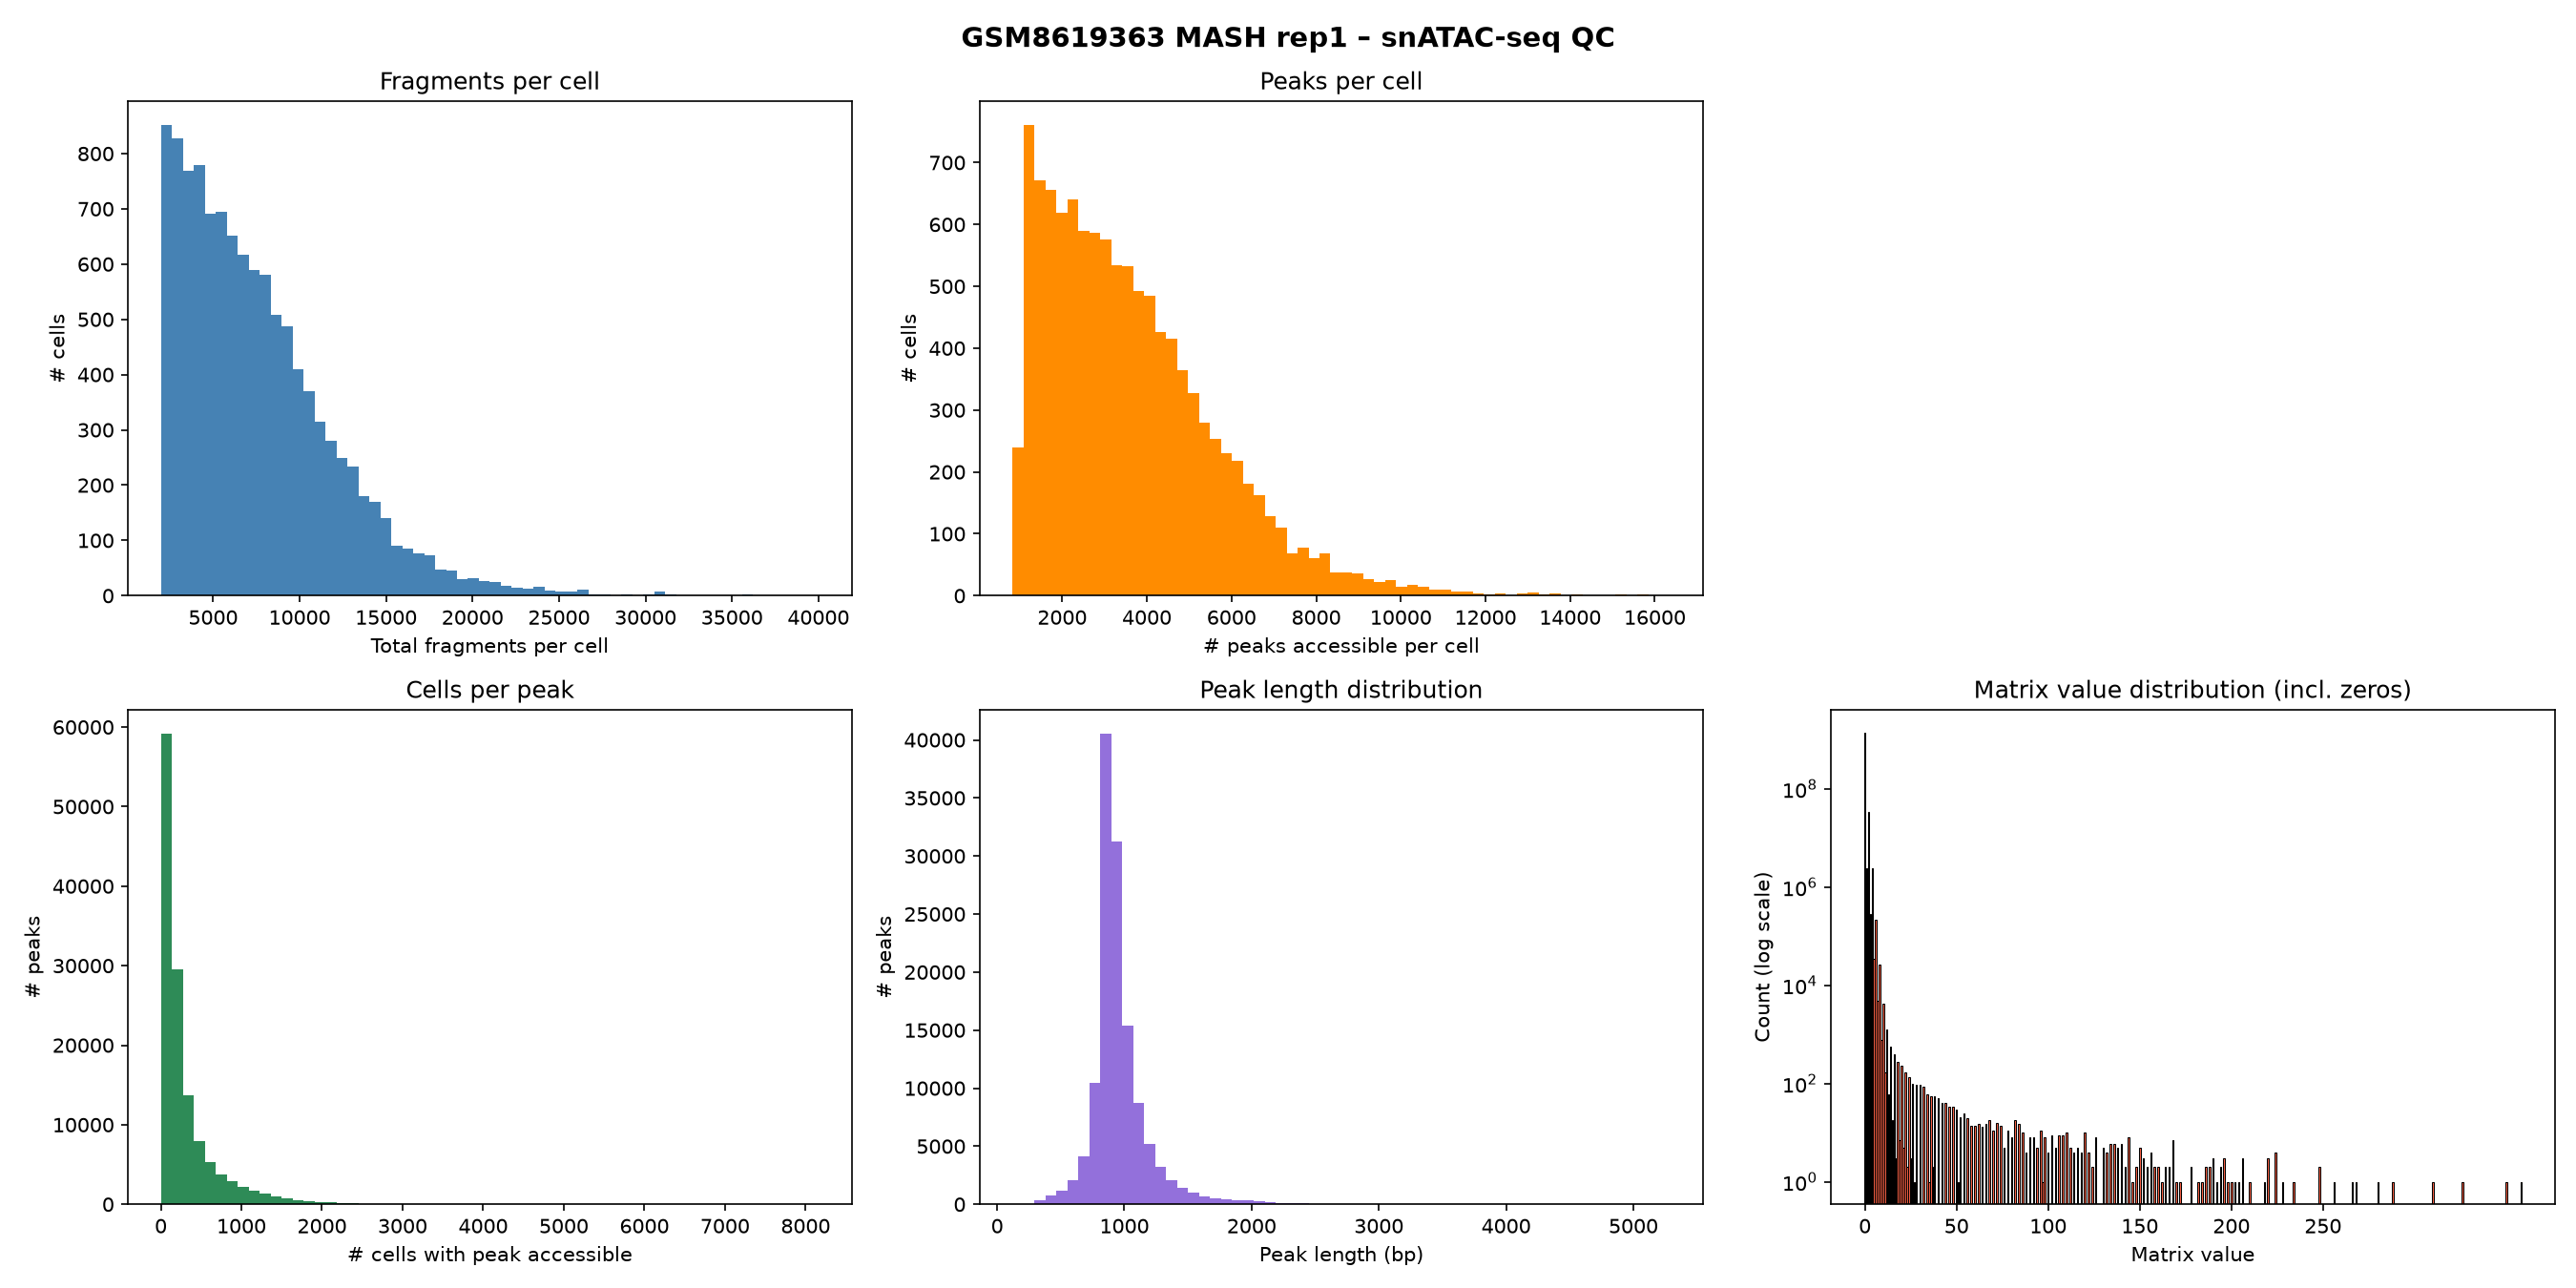
\includegraphics[width=\linewidth]{figres/snATAC_QC}
    \caption{Representative snATAC-seq quality-control summaries for a MASH sample. The panels show fragment depth per cell, accessible peaks per cell, cells per peak, peak length distribution, and matrix value distribution.}
    \label{fig:snatac-qc}
  \end{figure}

  \subsection{Differential Accessibility}\label{subsec:differential-accessibility}
  Differential accessibility was tested separately for each cell type using DESeq2\cite{Love2014DESeq2}.
  For each consensus peak, DESeq2 estimated the direction and magnitude of differential accessibility between healthy and MASH samples and adjusted for multiple testing.
  Peaks were selected using adjusted $p < 0.05$ and $|\log_2(\mathrm{FC})| \ge 0.58$, corresponding to at least about 1.5-fold change.

  After differential testing, we also examined sample-level consistency.
  For each selected peak, we returned to the pseudobulk counts and asked whether most biological samples supported the same direction of change, or whether the peak appeared to be driven by one unusually strong sample.
  This analysis is descriptive and does not replace DESeq2 significance, but it helps prioritize robust-looking signals.

  The strict significant-peak files were created by combining three filters.
  First, the peak had to pass the DESeq2 adjusted $p$-value threshold and the absolute effect-size threshold.
  Second, the median normalized accessibility had to agree with the DESeq2 direction: peaks with positive $\log_2(\mathrm{FC})$ should have larger MASH than healthy median accessibility, and peaks with negative $\log_2(\mathrm{FC})$ should show the reverse.
  Third, pairwise sample comparisons and leave-one-out recalculations had to remain directionally stable, while peaks dominated by a single sample were removed.
  This strict filtering step is why the final BED files contain fewer peaks than the broader DESeq2 diagnostic plots.

  Normalized counts were used only for this descriptive support filtering.
  Statistical significance and effect estimates came from DESeq2, while the sample-support layer acted as a guard against peaks whose significance was technically valid but visually or biologically fragile.

  \subsection{eQTL Filtering}\label{subsec:eqtl-filtering}
  We removed selected differential peaks that overlapped significant GTEx liver eQTL variants.
  This step intentionally makes the downstream question stricter: instead of rediscovering known eQTL-overlapping loci, the pipeline asks whether non-eQTL-overlapping differential accessibility peaks can still nominate coherent candidate genes.

  GTEx variant identifiers encode chromosome, position, reference allele, alternate allele, and genome build.
  We parsed those identifiers into one-base hg38 genomic intervals and removed any complete significant peak that overlapped at least one significant liver eQTL position.
  The filtering was performed per cell type, preserving valid empty BED files for cell types with no qualifying peaks.
  The resulting files in \href{https://github.com/noam-kimhi/Comp-Genomics-Hackathon/tree/main/data/derived/significant_peaks/filtered_significant_peaks}{\path{data/derived/significant_peaks/filtered_significant_peaks/}} are the peak files used for the main results in this report.

  \subsection{Peak-to-Gene Mapping}\label{subsec:peak-to-gene-mapping}
  The remaining peaks were mapped to genes using ABC predictions.
  ABC links candidate enhancers to genes using enhancer activity and chromatin contact information\cite{Fulco2019ABC}.
  Since the ABC file was in hg19, we used the UCSC liftover framework\cite{Kent2002UCSC} and intersected the lifted hg38 ABC intervals with our filtered peak set.
  A peak was considered mapped if it overlapped an ABC interval, and each peak-gene pair retained the ABC score as a confidence-like measure of enhancer-gene association.

  ABC mapping was many-to-many.
  A single peak can map to multiple genes when several ABC intervals overlap it, and a gene can be linked by more than one regulatory interval.
  We therefore reported both the number of mapped peaks and the number of peak-gene pairs.
  For interpretation, we prioritized genes with a clear biological relationship to MASLD, inflammation, fibrosis, or liver metabolism, while treating the ABC score as supportive rather than definitive evidence.

  \begin{figure}[H]
    \centering
    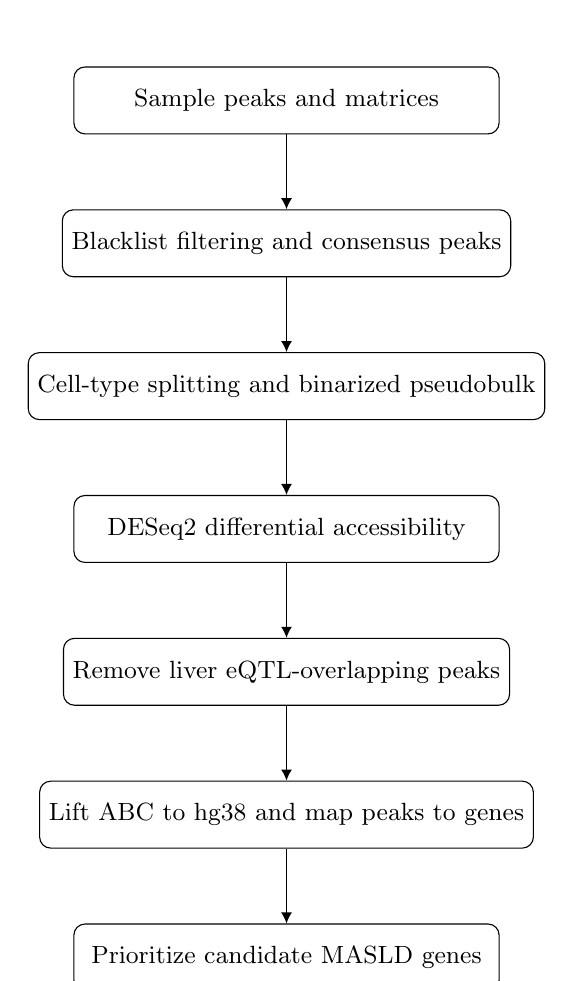
\begin{tikzpicture}[
      node distance=0.95cm,
      every node/.style={font=\small},
      box/.style={rectangle, draw, rounded corners, align=center, minimum width=5.4cm, minimum height=0.85cm},
      arrow/.style={-{Latex[length=1.4mm,width=1.4mm]}, line width=0.5pt}
    ]
      \node[box] (peaks) {Sample peaks and matrices};
      \node[box, below=of peaks] (consensus) {Blacklist filtering and consensus peaks};
      \node[box, below=of consensus] (split) {Cell-type splitting and binarized pseudobulk};
      \node[box, below=of split] (deseq) {DESeq2 differential accessibility};
      \node[box, below=of deseq] (eqtl) {Remove liver eQTL-overlapping peaks};
      \node[box, below=of eqtl] (abc) {Lift ABC to hg38 and map peaks to genes};
      \node[box, below=of abc] (genes) {Prioritize candidate MASLD genes};
      \draw[arrow] (peaks) -- (consensus);
      \draw[arrow] (consensus) -- (split);
      \draw[arrow] (split) -- (deseq);
      \draw[arrow] (deseq) -- (eqtl);
      \draw[arrow] (eqtl) -- (abc);
      \draw[arrow] (abc) -- (genes);
    \end{tikzpicture}
    \caption{Overview of the Hide and Peak analysis pipeline.}
    \label{fig:pipeline}
  \end{figure}

  \FloatBarrier

  \section{Results}\label{sec:results}

  \subsection{Differential Accessibility Is Concentrated in Specific Cell Types}\label{subsec:differential-accessibility-is-concentrated-in-specific-cell-types}
  The initial DESeq2 diagnostic output showed the strongest differential accessibility signal in Kupffer cells, followed by endothelial cells and hepatocytes.
  Before the strict sample-support filter, Kupffer cells had 92 DESeq2-selected peaks, split almost evenly between peaks more accessible in healthy samples (44) and peaks more accessible in MASH samples (48).
  The strict filtered files used for downstream eQTL filtering and ABC mapping are reported in the next subsection.

  \begin{figure}[H]
    \centering
    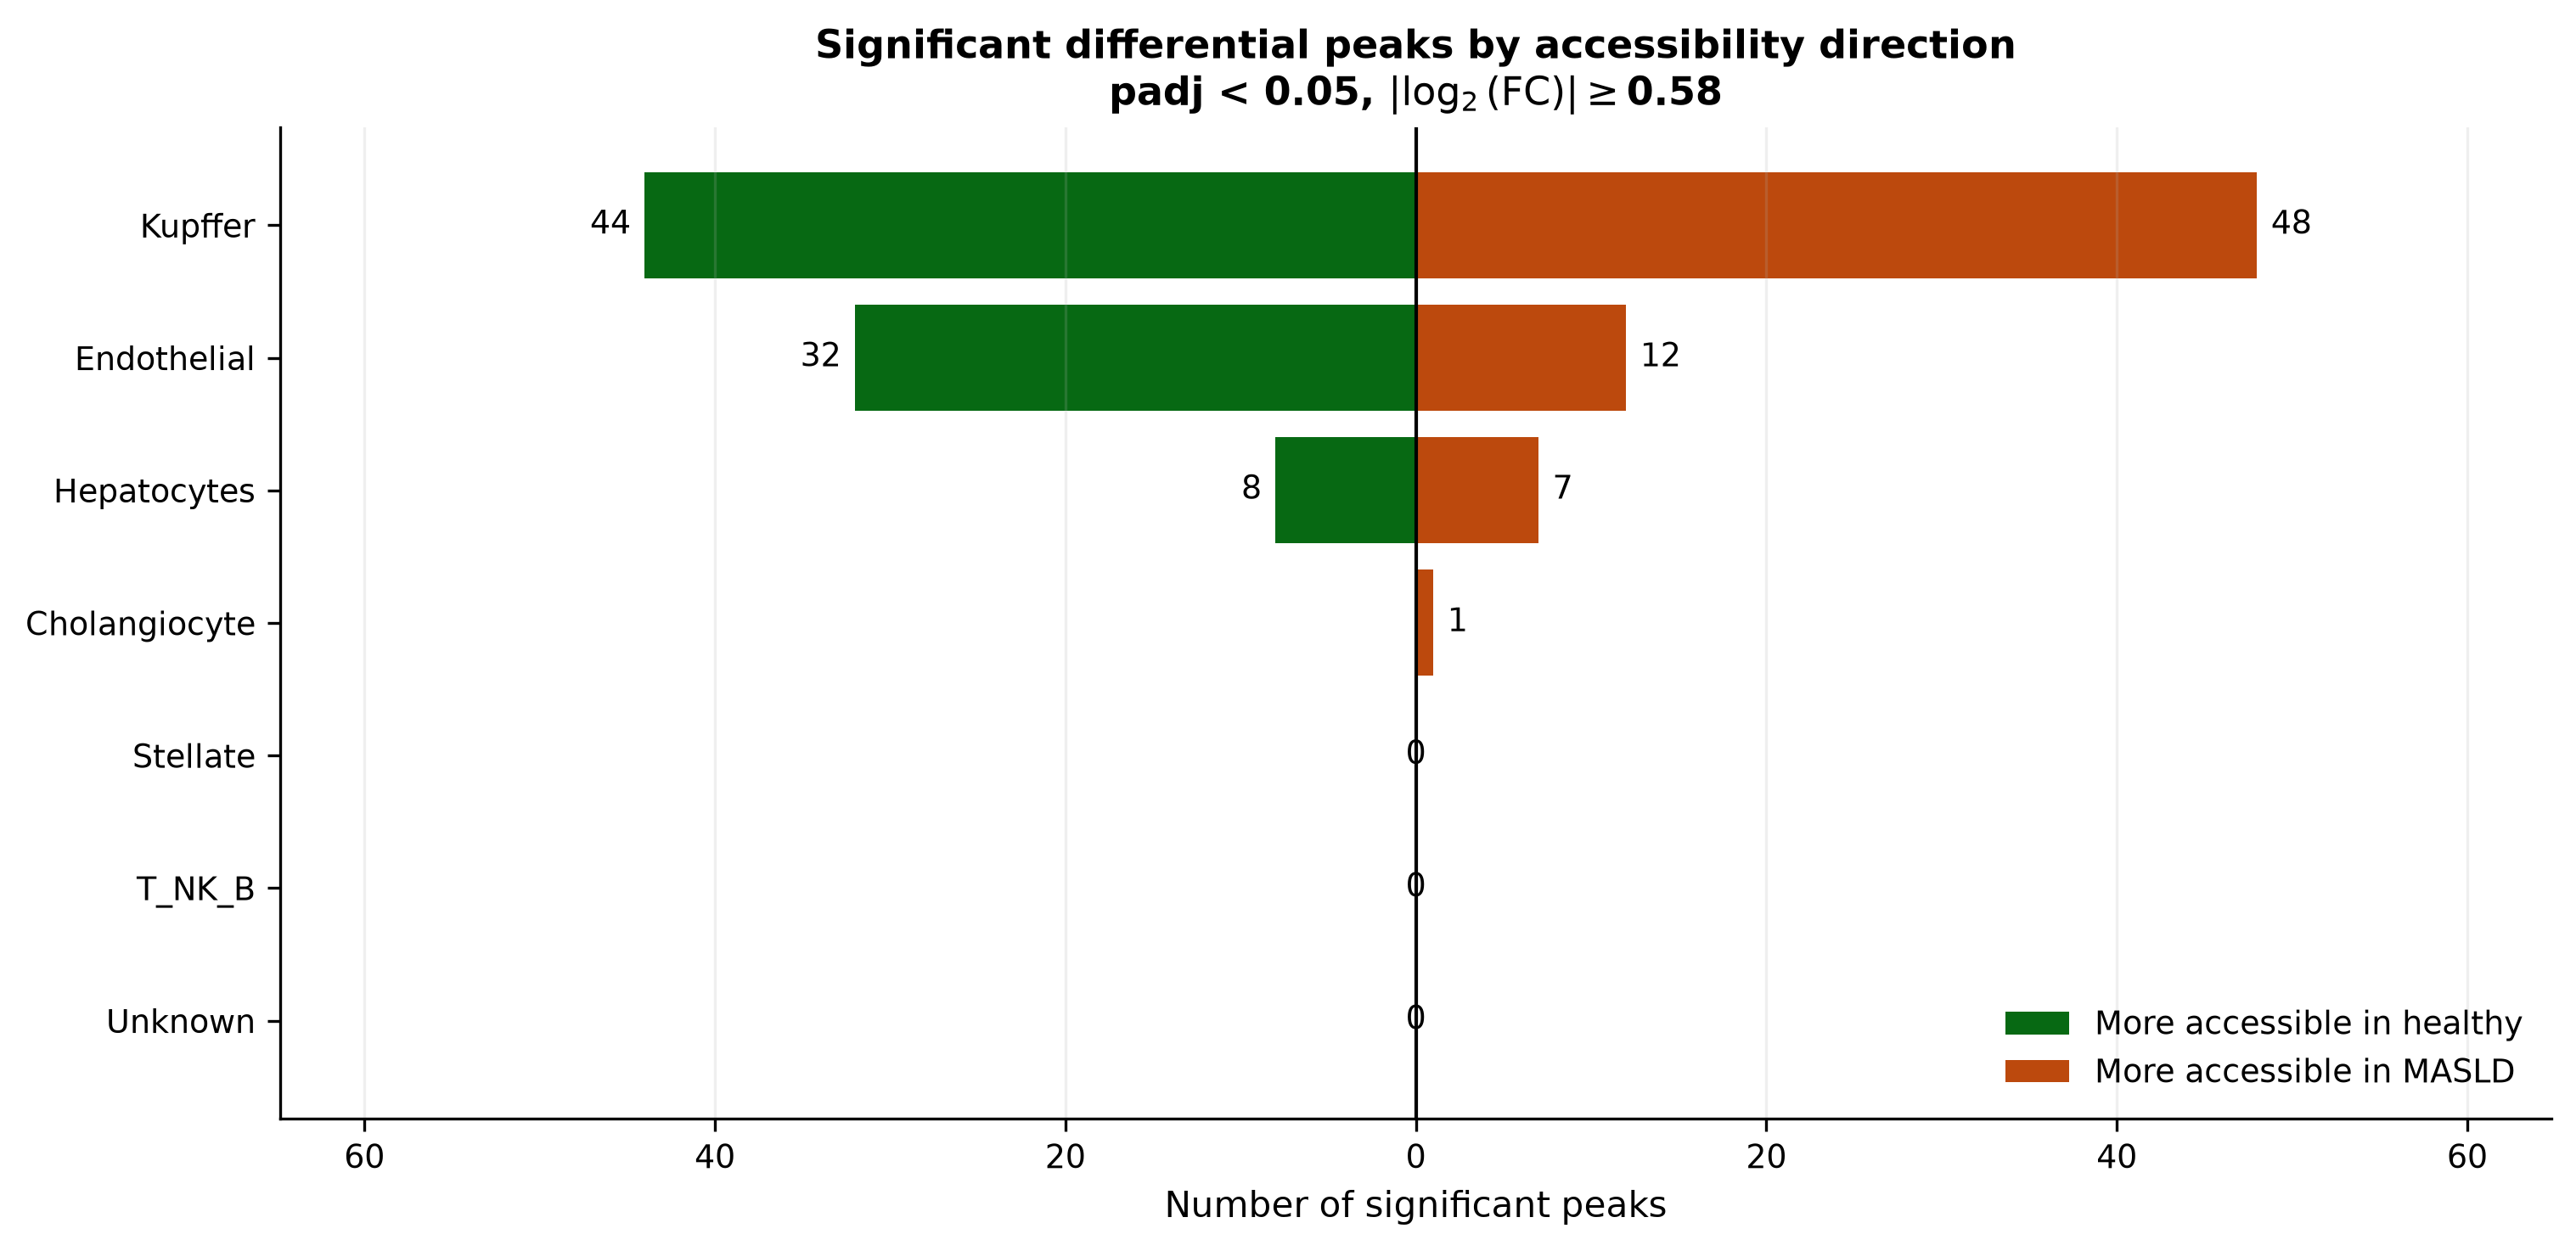
\includegraphics[width=0.88\linewidth]{figres/all_cell_types_significant_direction_counts}
    \caption{DESeq2 diagnostic view of differentially accessible peaks by cell type and direction before the strict sample-support filter. Green bars indicate peaks more accessible in healthy samples, and orange bars indicate peaks more accessible in MASH samples.}
    \label{fig:direction-counts}
  \end{figure}

  Kupffer cells are liver-resident macrophages, so their dominance in the results suggests that the accessibility signal captures immune and inflammatory components of MASH rather than only hepatocyte-intrinsic regulation.
  This is consistent with the biological expectation that MASH progression involves inflammatory signaling, macrophage activation, and fibrosis-related tissue remodeling.

  \begin{figure}[H]
    \centering
    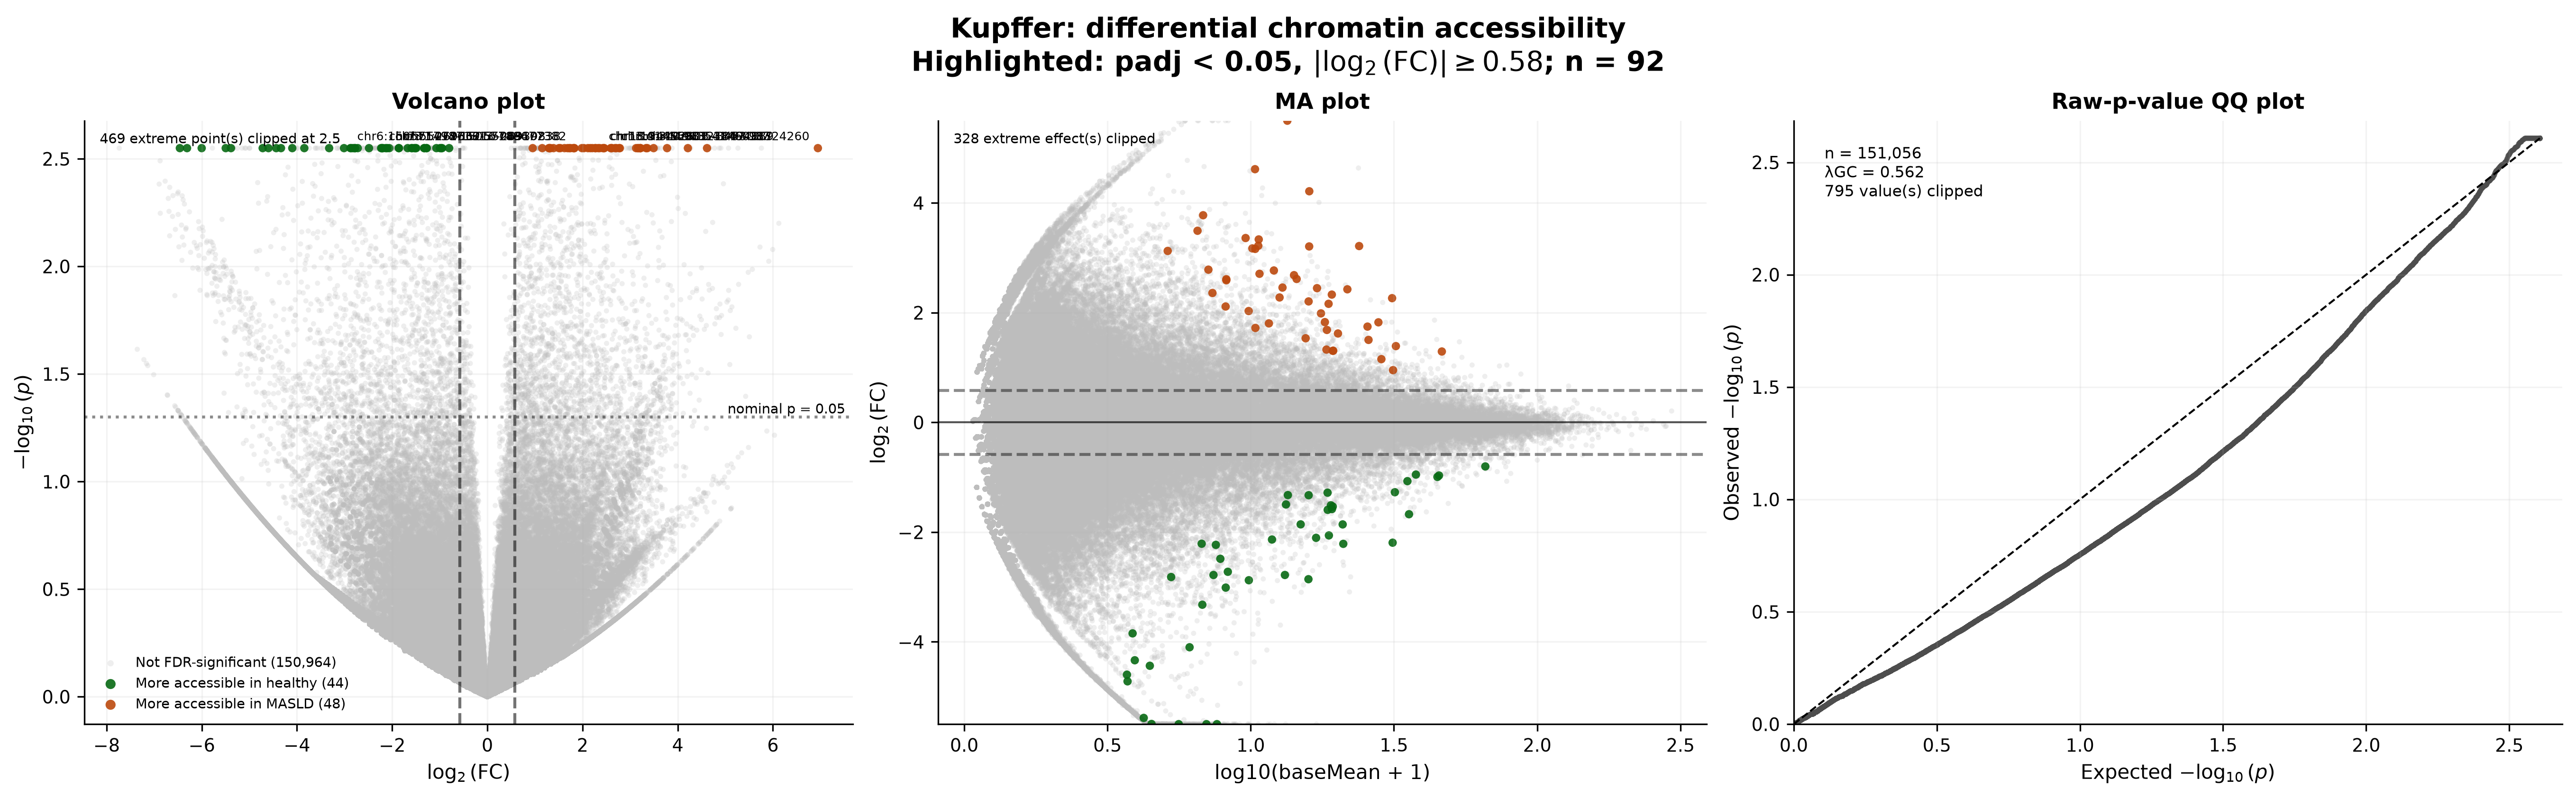
\includegraphics[width=\linewidth]{figres/Kupffer_differential_accessibility_dashboard}
    \caption{Kupffer-cell differential accessibility dashboard. The volcano and MA plots show selected differential peaks in orange or green according to direction, while the QQ plot summarizes raw $p$-value behavior.}
    \label{fig:kupffer-da}
  \end{figure}

  \subsection{Filtering Known Liver eQTL Overlaps Retains Candidate Signal}\label{subsec:filtering-known-liver-eqtl-overlaps-retains-candidate-signal}
  In the strict filtered set used for the main analysis, Kupffer cells had 61 high-confidence significant peaks, of which 10 overlapped significant liver eQTL variants and 51 remained after eQTL filtering.
  Endothelial cells retained 27 of 34 peaks, hepatocytes retained 10 of 12, and cholangiocytes retained its single selected peak.
  These results show that most high-confidence peaks in the main signal-bearing cell types did not overlap the significant liver eQTL catalogue used here.

  \begin{table}[H]
    \centering
    \small
    \begin{tabular}{lcccc}
      \toprule
      Cell type & Selected peaks & eQTL-overlap removed & Remaining peaks & Fraction removed \\
      \midrule
      Cholangiocyte & 1 & 0 & 1 & 0.00 \\
      Endothelial & 34 & 7 & 27 & 0.21 \\
      Hepatocytes & 12 & 2 & 10 & 0.17 \\
      Kupffer & 61 & 10 & 51 & 0.16 \\
      Stellate & 0 & 0 & 0 & 0.00 \\
      T/NK/B & 0 & 0 & 0 & 0.00 \\
      Unknown & 0 & 0 & 0 & 0.00 \\
      \bottomrule
    \end{tabular}
    \caption{Strict filtered significant peaks before and after removing peaks overlapping significant liver eQTL variants.}
    \label{tab:eqtl-filter}
  \end{table}

  \begin{figure}[H]
    \centering
    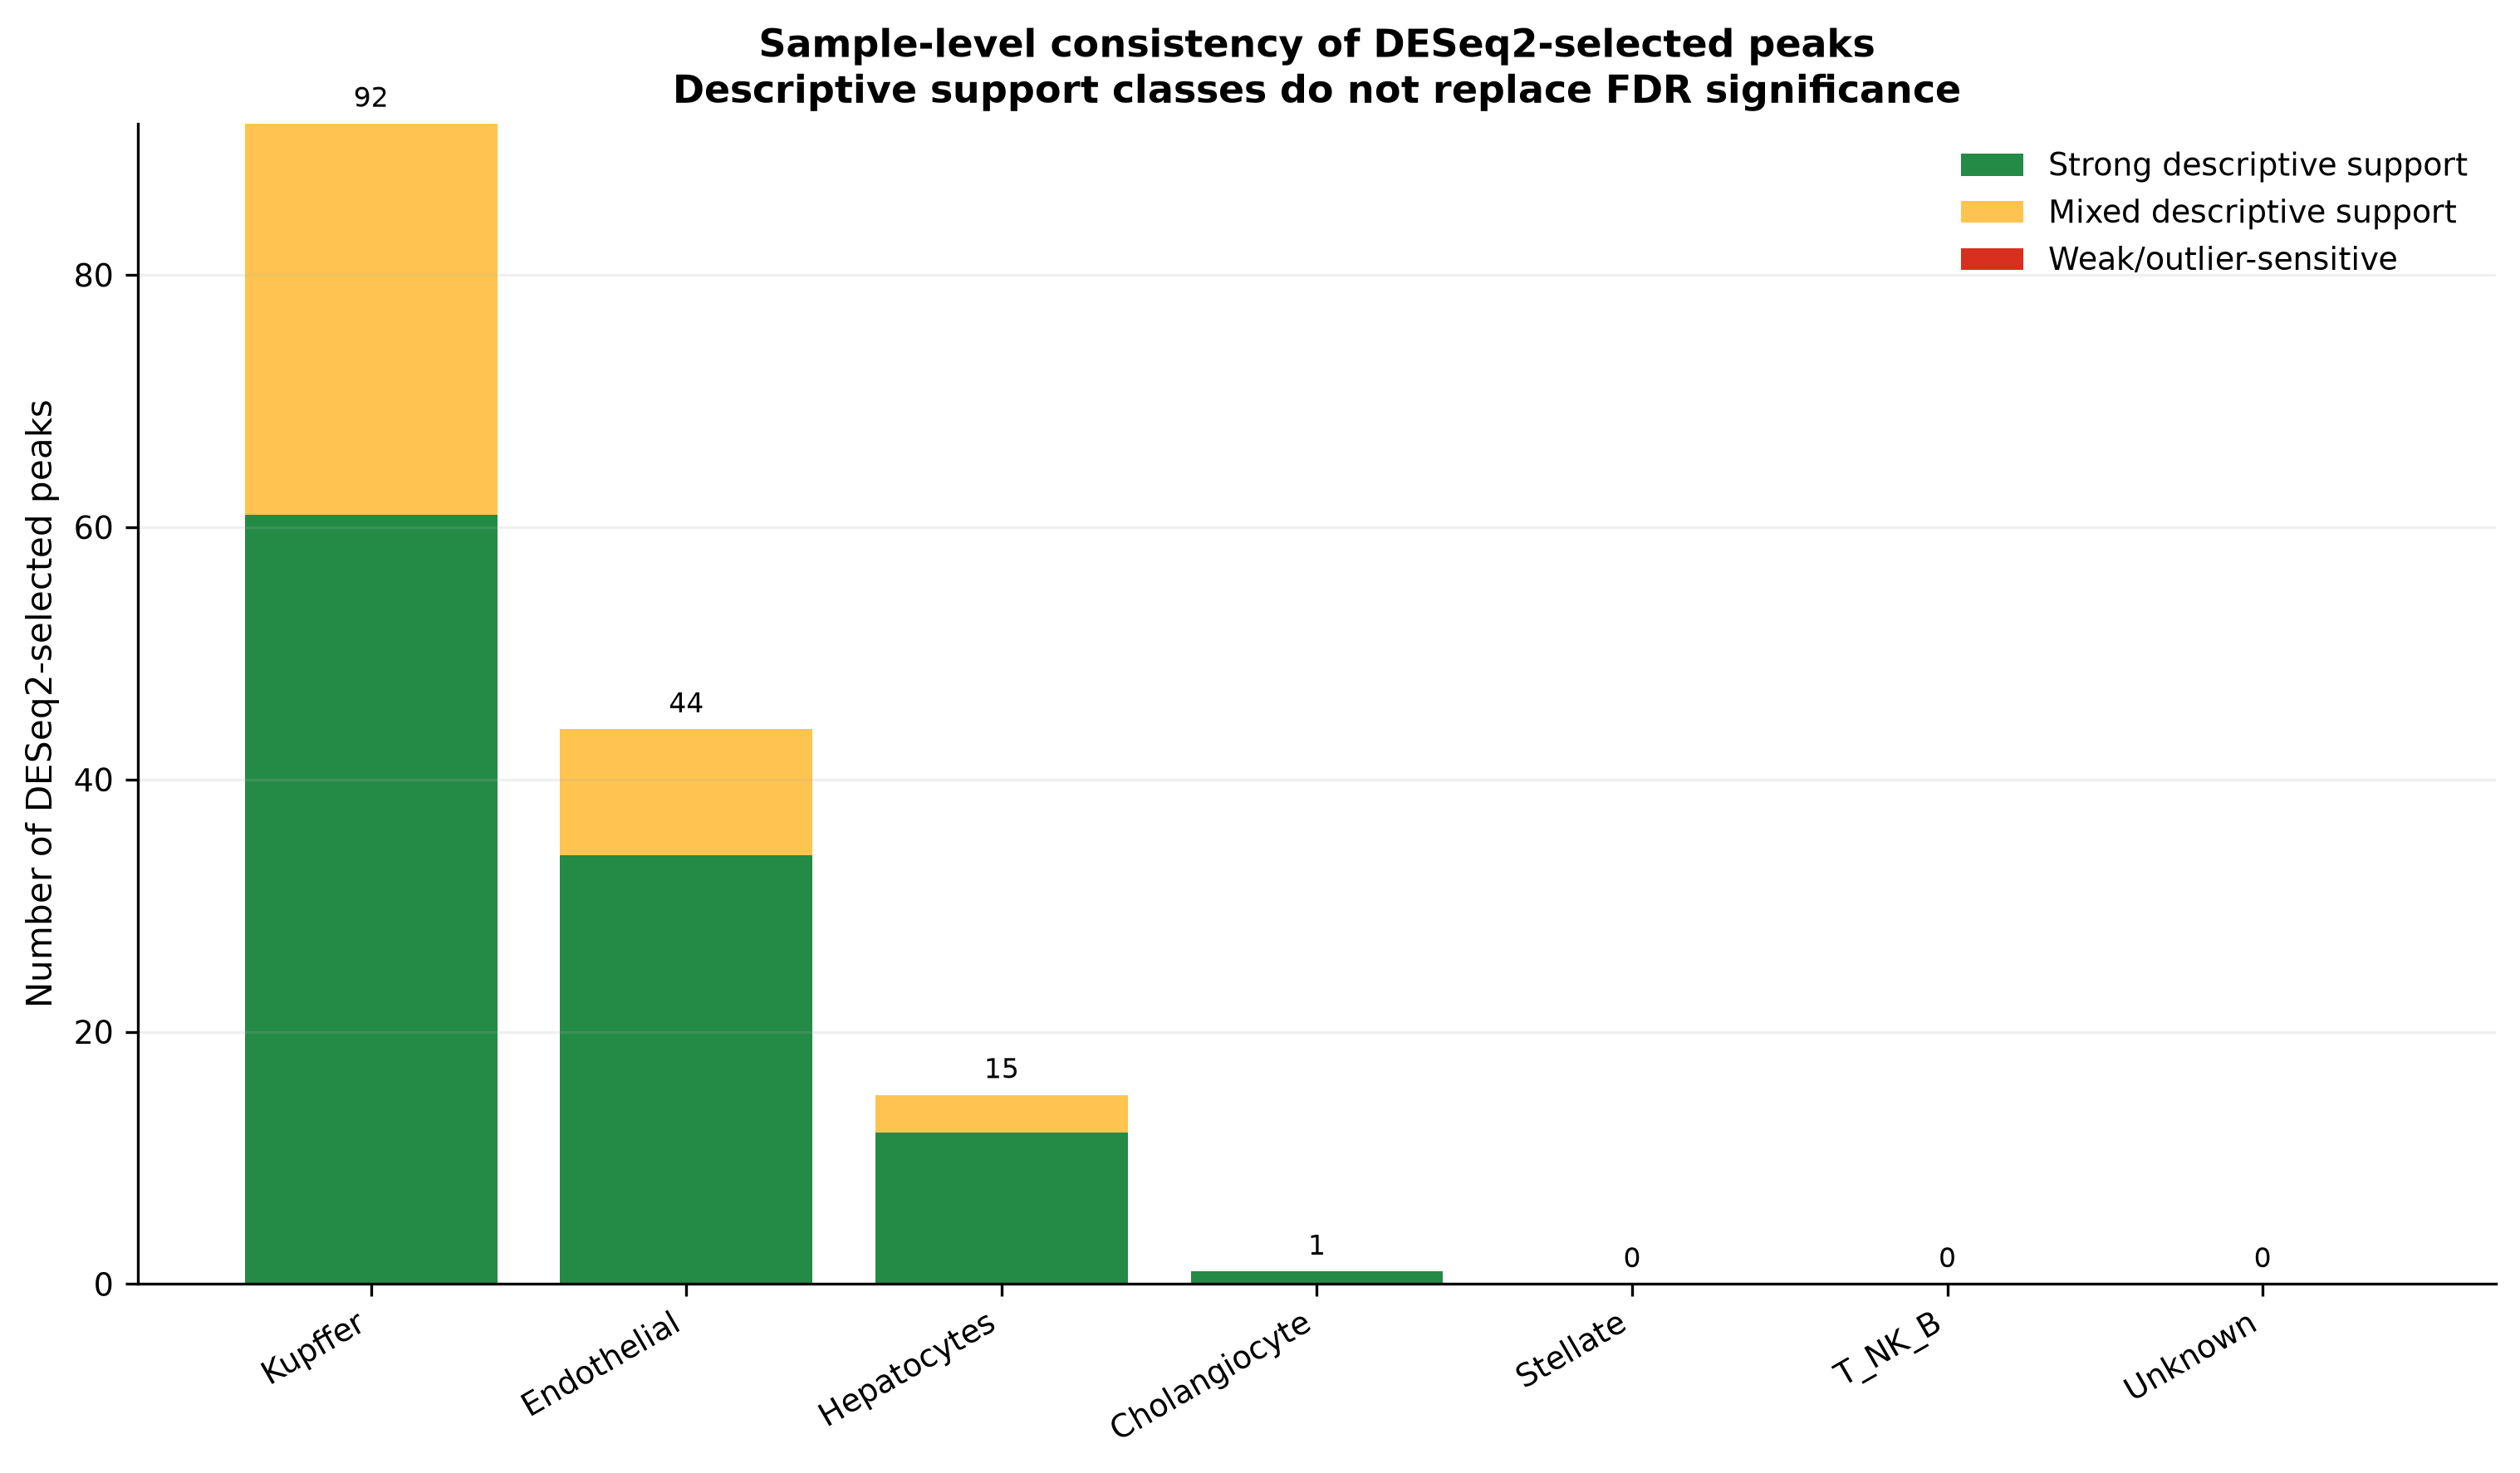
\includegraphics[width=0.88\linewidth]{figres/all_cell_types_candidate_sample_support}
    \caption{Sample-level consistency classes for the broader DESeq2-selected diagnostic set. The strict filtered BED files used downstream retain the high-confidence subset after applying sample-support criteria.}
    \label{fig:sample-support}
  \end{figure}

  \subsection{ABC Mapping Prioritizes Kupffer-Cell Candidate Genes}\label{subsec:abc-mapping-prioritizes-kupffer-cell-candidate-genes}
  After eQTL filtering, ABC mapping produced the richest peak-gene set in Kupffer cells: 17 of 51 remaining Kupffer peaks mapped to 40 peak-gene pairs.
  Endothelial cells had 9 mapped peaks and 21 peak-gene pairs, hepatocytes had one mapped peak and one pair, and cholangiocytes had one mapped peak and one pair.
  This again points to Kupffer cells as the strongest source of interpretable candidate genes in the current analysis.

  \begin{table}[H]
    \centering
    \small
    \begin{tabular}{lccc}
      \toprule
      Cell type & Peaks after eQTL filtering & ABC-mapped peaks & Peak-gene pairs \\
      \midrule
      Cholangiocyte & 1 & 1 & 1 \\
      Endothelial & 27 & 9 & 21 \\
      Hepatocytes & 10 & 1 & 1 \\
      Kupffer & 51 & 17 & 40 \\
      Stellate & 0 & 0 & 0 \\
      T/NK/B & 0 & 0 & 0 \\
      Unknown & 0 & 0 & 0 \\
      \bottomrule
    \end{tabular}
    \caption{ABC mapping summary for the strict filtered peak set.}
    \label{tab:abc-summary}
  \end{table}

  We focused on biologically interpretable candidates highlighted by the strict ABC-mapped results.
  Candidate prioritization considered four pieces of evidence together: whether the peak survived the strict non-eQTL filtering, the DESeq2 effect size and adjusted significance, the sample-support label, and whether the ABC target gene had a plausible relationship to MASLD, inflammation, fibrosis, or liver-cell biology.
  This is important because no single score is sufficient on its own.
  For example, a high ABC score is useful only if the accessibility signal is robust, while a biologically famous gene is less convincing if the regulatory link is weak or the peak is driven by one sample.
  The main examples are summarized in \cref{tab:candidates}.

  \begin{table}[H]
    \centering
    \scriptsize
    \begin{tabularx}{\linewidth}{l l X c l X}
      \toprule
      Gene & Cell & Peak & ABC & Direction & Interpretation \\
      \midrule
      GSDME/DFNA5 & Kupffer & chr7:24756018--24758867 & 0.462 & MASH & Pyroptosis/inflammation \\
      RGCC & Kupffer & chr13:41455801--41460317 & 0.216 & MASH & Disease-state marker \\
      SHP/NR0B2 & Kupffer & chr1:26936216--26939838 & 0.020 & Healthy & Protective nuclear receptor \\
      SMAD2 & Endothelial & chr18:48001672--48005584 & 0.043 & MASH & TGF-\(\beta\)/fibrosis signaling \\
      \bottomrule
    \end{tabularx}
    \caption{Selected non-eQTL-overlapping peak-to-gene candidates. GSDME appears in the ABC-derived tables under its older symbol, DFNA5; SHP appears as NR0B2.}
    \label{tab:candidates}
  \end{table}

  \subsubsection{GSDME/DFNA5}
  The strongest ABC-scored candidate in the highlighted results was a Kupffer-cell peak at chr7:24756018--24758867 linked to \textit{DFNA5}, the older name for \textit{GSDME}, with ABC score 0.462.
  This peak was more accessible in MASH and had strong sample-level descriptive support in the project output.
  The DESeq2 result for Kupffer cells showed $\log_2(\mathrm{FC}) = 2.33$, adjusted $p = 0.0072$.
  The effect is therefore not only statistically significant but also large in magnitude: the accessibility signal points to a several-fold increase in MASH Kupffer cells.
  The same peak remained after removing known significant liver eQTL overlaps, which makes it especially useful for our research question because it represents a disease-associated accessibility signal that is not simply a rediscovery of a known liver eQTL position.

  The ABC evidence is also unusually strong for this candidate.
  The linked ABC interval overlaps the consensus peak and assigns the peak to \textit{DFNA5}/\textit{GSDME} with the highest score among the highlighted candidates.
  In the local ABC dictionary, nearby liver and hepatocyte annotations also support this region as a regulatory neighborhood for \textit{DFNA5}/\textit{GSDME}, which increases our confidence that the peak-to-gene assignment is not arbitrary.

  GSDME is a compelling biological match because recent work reports that GSDME promotes MASLD through pyroptosis, mitochondrial dynamics, and energy-balance effects in intestine and liver\cite{Zhu2024GSDME}.
  This gives the result a coherent direction: MASH is the inflammatory form of metabolic liver disease, Kupffer cells are liver-resident macrophages, and GSDME is connected to inflammatory cell death.
  In our context, increased accessibility near a GSDME-linked regulatory element in Kupffer cells is therefore consistent with an inflammatory macrophage-mediated contribution to MASH progression.
  We do not claim that this peak proves \textit{GSDME} activation in Kupffer cells, but among the current candidates it is the clearest convergence of effect size, enhancer-gene score, cell type, and disease literature.

  \subsubsection{RGCC}
  A second Kupffer-cell MASH-accessible peak at chr13:41455801--41460317 mapped to \textit{RGCC} with ABC score 0.216.
  This peak had the strongest statistical support among the highlighted Kupffer candidates, with $\log_2(\mathrm{FC}) = 2.43$ and adjusted $p = 2.3 \times 10^{-5}$.
  It also received strong descriptive support in the sample-level analysis, meaning that the MASH direction was not just a single-sample artifact.
  Together, these properties make the \textit{RGCC}-linked peak one of the most robust accessibility changes in the final mapped set.

  RGCC is not necessarily a proven causal driver of MASH, but it has been implicated in MASLD diagnostic modeling and appears in a gene-discovery context associated with clinical validation and mechanism exploration\cite{Wang2024RGCC}.
  This distinction matters for interpretation.
  Unlike GSDME, where there is a more direct mechanistic connection to MASLD-related inflammatory damage, \textit{RGCC} is better viewed as a disease-associated candidate whose relevance may reflect inflammatory state, immune infiltration, or broader tissue remodeling.

  The strength of the \textit{RGCC} result is therefore mainly empirical.
  It survived the strict filtering, mapped with a moderate ABC score, and showed a large MASH-associated Kupffer-cell accessibility increase.
  Because Kupffer cells dominate the interpretable part of our results, a robust \textit{RGCC}-linked macrophage-region is worth reporting even if the gene's role in MASH is less settled than that of GSDME or SHP.
  In our results, \textit{RGCC} is best interpreted as a plausible disease-state or immune-environment marker rather than a mechanistically established regulator.

  \subsubsection{SHP/NR0B2}
  The SHP candidate appears as \textit{NR0B2} in the peak-to-gene table.
  A Kupffer-cell peak at chr1:26936216--26939838 mapped to \textit{NR0B2} with ABC score 0.020 and was more accessible in healthy samples.
  The accessibility direction is the central reason this candidate is interesting.
  The DESeq2 result showed $\log_2(\mathrm{FC}) = -1.86$ with adjusted $p = 4.7 \times 10^{-4}$, so the peak is substantially less accessible in MASH than in healthy Kupffer cells.
  The sample-support analysis also labeled this peak as strongly supported, suggesting that the healthy-accessible pattern is reproducible across samples after the strict filtering step.

  Although its ABC score is modest, the direction is biologically meaningful: SHP has been shown to suppress inflammation and fibrosis in a mouse model of nonalcoholic steatohepatitis\cite{Zou2018SHP}.
  In other words, the result points in the opposite direction from GSDME and RGCC.
  Rather than nominating a region that becomes more open in disease, it nominates a region linked to a protective nuclear receptor that is more accessible in healthy samples.
  This gives a plausible loss-of-protection interpretation: MASH may involve reduced accessibility at a regulatory element connected to anti-inflammatory or anti-fibrotic signaling.

  This candidate also illustrates why we should not rank results by ABC score alone.
  The \textit{NR0B2} ABC score is lower than the other highlighted candidates, but the direction of accessibility and the prior biology make it highly interpretable.
  We therefore include it not as the strongest enhancer-gene prediction, but as a biologically coherent candidate whose decreased accessibility matches a known protective role for SHP in NASH-like liver injury.

  \subsubsection{SMAD2}
  We also identified an endothelial-cell peak at chr18:48001672--48005584 linked to \textit{SMAD2} with ABC score 0.043.
  This peak was more accessible in MASH, had strong descriptive support, and showed one of the larger endothelial-cell effects in the strict mapped set: $\log_2(\mathrm{FC}) = 2.41$, adjusted $p = 0.028$.
  Although the endothelial signal was smaller overall than the Kupffer-cell signal, this candidate is valuable because it broadens the results beyond macrophage-centered inflammation.
  The mapped peak suggests that disease-associated chromatin remodeling may also appear in liver endothelial cells, a compartment relevant to sinusoidal structure, immune-cell recruitment, vascular stress, and fibrotic remodeling.

  \textit{SMAD2} is a receptor-regulated mediator of TGF-\(\beta\) signaling, a pathway repeatedly implicated in liver-disease progression, fibrogenesis, and NAFLD progression\cite{Dooley2012TGFB,Nair2020TGFBNAFLD}.
  This makes the peak-to-gene result particularly interpretable despite the moderate ABC score.
  TGF-\(\beta\)/SMAD signaling is one of the canonical pathways connecting chronic liver injury to fibrosis, and endothelial dysfunction can interact with inflammatory and fibrotic programs during liver-disease progression.
  A MASH-accessible endothelial peak linked to \textit{SMAD2} therefore fits the broader biology of disease-associated tissue remodeling.

  We include \textit{SMAD2} as a pathway-consistent candidate rather than as direct proof of endothelial \textit{SMAD2} regulation.
  Its value in the report is that it shows the pipeline can recover candidates outside the dominant Kupffer-cell axis and connect them to an established profibrotic signaling pathway.
  Follow-up analyses could test whether this region overlaps endothelial enhancer marks, whether \textit{SMAD2} expression changes in matched single-cell RNA-seq data, or whether the same locus appears in fibrosis-associated endothelial states.

  \FloatBarrier

  \section{Discussion}\label{sec:discussion}

  \subsection{Summary}\label{subsec:summary}
  We built a cell-type-aware pipeline for finding MASLD-associated regulatory peaks that are not already explained by significant liver eQTL overlap.
  The main signal emerged in Kupffer cells, where the strict pipeline identified 61 high-confidence significant peaks, retained 51 after eQTL filtering, and mapped 17 of those peaks to 40 ABC peak-gene pairs.
  Among the highlighted candidates, GSDME/DFNA5, RGCC, and SMAD2 were linked to peaks more accessible in MASH, while SHP/NR0B2 was linked to a peak more accessible in healthy samples.

  \subsection{Analysis}\label{subsec:analysis}
  The results support the central hypothesis: non-eQTL-overlapping chromatin accessibility peaks can still nominate biologically plausible MASLD genes.
  The strongest example is GSDME/DFNA5, whose MASH-accessible Kupffer-cell peak maps with a high ABC score and is supported by recent literature connecting GSDME to MASLD and pyroptosis.
  The SHP/NR0B2 result is interesting for the opposite reason: a protective anti-inflammatory factor is linked to a healthy-accessible peak, matching a model in which loss of protective regulatory accessibility may contribute to disease.
  SMAD2 broadens the candidate set beyond Kupffer cells, suggesting that endothelial regulatory remodeling may also connect to profibrotic TGF-\(\beta\) signaling.

  The analysis also shows why cell-type resolution matters.
  If all liver nuclei were aggregated together, immune-cell-specific regulatory signals could be diluted by hepatocyte-dominated accessibility.
  By splitting the matrices by cell type before pseudobulk testing, the pipeline recovered a Kupffer-cell-centered signal that aligns well with inflammatory biology in MASH.

  \subsection{Limitations}\label{subsec:limitations}
  The project should be interpreted as candidate prioritization, not causal proof.
  DESeq2 identifies differential accessibility, ABC predicts enhancer-gene links, and literature support provides plausibility; none of these steps demonstrates that the peak regulates the gene in Kupffer cells or that the gene causally drives MASH.

  There are also data and modeling limitations.
  Effective replicate support varied across cell types, and some sample-cell-type combinations had no data.
  The eQTL filter depends on the completeness and tissue context of the GTEx liver eQTL catalogue; absence from this catalogue does not mean absence of regulatory evidence in every possible dataset.
  ABC links were derived from external liver-related regulatory resources and then lifted from hg19 to hg38, so coordinate handling and tissue-context mismatch are important caveats even though the liftover mapping rate was high.

  \subsection{Future Work}\label{subsec:future-work}
  The next step is to validate the peak-to-gene links using cell-type-specific chromatin-contact data or perturbation experiments such as CRISPRi. The analysis could also be extended by modeling disease-associated cell states within broad cell types, rather than treating each cell type as homogeneous. Finally, an enrichment test could ask whether genes nominated by the pipeline are enriched for known MASLD, inflammation, fibrosis, or lipid-metabolism genes compared with an appropriate background of ABC-mappable genes.

  \FloatBarrier
  \newpage

  \bibliographystyle{unsrturl}
  \bibliography{references}

\end{document}
